%\subsection{Aplicativo}

	\par Para iniciar a construção do aplicativo, fez-se necessário a instalação e
configuração do ambiente de desenvolvimento. Primeiramente, realizou-se o
\textit{download} da IDE \textit{Android Studio}, versão {1.1.0} e do
\textit{Android} SDK, versão {24.0.2}, ambos no site \textit{Developers
Android}.

	\par Contudo, ao executar o emulador do \textit{Android} o sistema apresentava
a seguinte mensagem: \textit{“emulator: Failed to open the HAX device!”}.
Depois de algum tempo pesquisando, percebeu-se que era necessário instalar um
programa chamado \textit{Intel Hardware Accelerated Execution Manager} (HAXM),
responsável por aumentar a performance do emulador.

	\par No entanto, ao instalá-lo ocorria o seguinte erro: "\textit{this computer
meets the requirements for haxm but intel virtualization technology (VT-x) is
not turned on}". A solução foi acessar a BIOS da máquina e habilitar o
assistente de \textit{hardware} para virtualização. Daí em diante, foi possível
executar no emulador as aplicações feitas no \textit{Android Studio}.

	\par Com o ambiente já configurado, criou-se um repositório no controlador de
versão \textit{Github}, cujo todos os participantes possuem acesso, para que
ambos tenham a versão mais recente do aplicativo em seu dispositivo.

	\par A partir de então, passou-se a desenvolver o \textit{software}. A
princípio, foi construída uma \texttt{activity}, que é acessível ao aluno logo
que a aplicação se inicia. Essa \texttt{activity} é do tipo \textit{Navigation
Drawer Layout}, ou seja, é um painel que permite inserir as opções de navegação
do aplicativo, semelhante a um menu.

	\par Ao criar essa \texttt{activity}, o \textit{Android Studio} gera
automaticamente a classe \texttt{NavigationDrawerFragment} e um arquivo XML na
pasta \texttt{layout}, chamado \texttt{fragment\_navigation\_drawer.xml}.

	\par No arquivo \texttt{fragment\_navigation\_drawer.xml} foram inseridos três
\textit{widgets}, sendo dois do tipo \texttt{textView}, para o cabeçalho com a
logomarca da Univás e para o rodapé com o seguinte texto: "Univás - Pouso
Alegre - MG" e um \textit{widget} do tipo \texttt{listView} que contém a lista
com as opções que o \textit{software} oferece ao aluno. Na Figura
\ref{fig:aplicativo}, podem ser vistos os \textit{widgets} no arquivo
\texttt{fragment\_navigation\_drawer.xml}

	\begin{figure}[h!] 
		\centerline{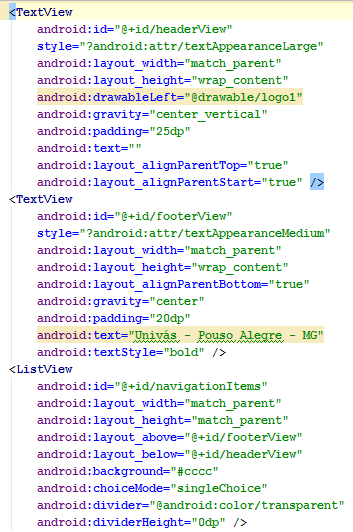
\includegraphics[scale=0.7]{./imagens/2_q_metodologico/4_procedimentos_resultados/42_aplicativo/aplicativo.png}}
		\caption[sem legenda]{sem legenda. \textbf{Fonte:}Elaborado pelos autores.}
		\label{fig:aplicativo}
	\end{figure}
	
	\pagebreak
	
	\par A classe \texttt{NavigationDrawerFragment} representa o painel de
navegação. Nela se destacam os métodos \texttt{onCreateView()}, responsável por
criar o \textit{layout} de navegação e o \texttt{selectItem()}, encarregado em
identificar qual item foi escolhido pelo usuário. Na figura
\ref{fig:aplicativo1}, vê-se o método \texttt{onCreateView()}, informando ao
sistema operacional o \textit{layout} a ser chamado e adicionando a um
\texttt{array} de \textit{String} as alternativas de navegação que serão
exibidos no \texttt{listView} do arquivo
\texttt{fragment\_navigation\_drawer.xml}.


	\begin{figure}[h!] 
		\centerline{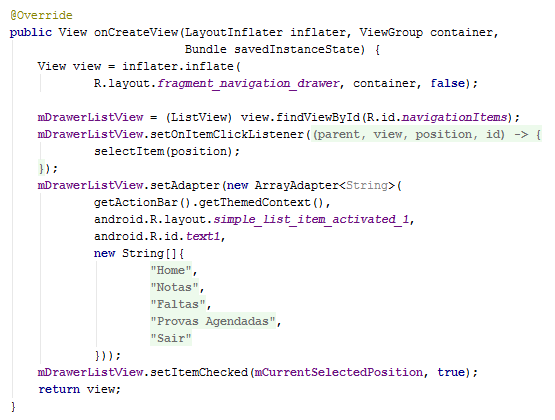
\includegraphics[scale=0.7]{./imagens/2_q_metodologico/4_procedimentos_resultados/42_aplicativo/aplicativo1.png}}
		\caption[sem legenda]{sem legenda. \textbf{Fonte:}Elaborado pelos autores.}
		\label{fig:aplicativo1}
	\end{figure}
	
	\pagebreak
	
	\par O próximo passo, foi criação de uma \texttt{activity} do tipo
\texttt{blank activity} com finalidade de listar as notas. Ao criá-la com o
nome de \texttt{ListResultsActivity}, o \textit{Android Studio} gera dentro da
pasta \textit{layout} o arquivo XML referente a ela, chamado de
\texttt{activity\_list\_results.xml}. Neste, foi inserido apenas o
\textit{widget} \texttt{expandableListView}, que está incumbido de apresentar a
lista de disciplinas cujo o discente está cursando e ao clicar em alguma dessas
matérias serão apresentadas as notas referentes aos exercícios realizados desta
disciplina. Na Figura \ref{fig:aplicativo2} é possível ver o \textit{layout} com uma
lista do tipo \texttt{expandableListView}.


	\begin{figure}[h!] 
		\centerline{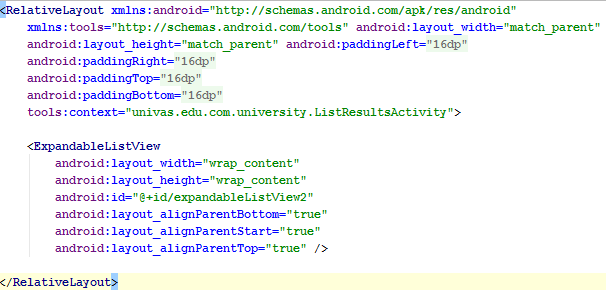
\includegraphics[scale=0.7]{./imagens/2_q_metodologico/4_procedimentos_resultados/42_aplicativo/aplicativo2.png}}
		\caption[sem legenda]{sem legenda. \textbf{Fonte:}Elaborado pelos autores.}
		\label{fig:aplicativo2}
	\end{figure}
	
	\pagebreak
	
	\par Depois, fez-se necessário a criação de uma classe encarregada por
organizar e controlar todas as atualizações dos itens de uma lista. Essa classe
recebeu o nome de \texttt{ListResultsAdapter} e estende da classe
\texttt{BaseExpandableListAdapter}, nativa do \textit{Android}.

	\par Os procedimentos acima citados foram necessários também para as opções de
faltas e provas agendadas. Após construídos todos os \textit{layouts}, foi
fundamental criar o banco de dados, no qual o aplicativo salva as informações
recebidas do \textit{web service}. Para que isso fosse possível, elaborou-se
uma classe denominada \texttt{DatabaseHelper} que estende da classe
\texttt{SQLiteOpenHelper} do \textit{Android}, com dois métodos, um chamado
\texttt{onCreate()} e outro conhecido por \texttt{onUpgrade()}.

	\par Foi preciso criar um atributo que mantém a versão do banco de dados. Essa
informação serve para que o \textit{Android} consiga saber qual dos dois
métodos devem ser executados. Ao iniciar a aplicação pela primeira vez, estando
a versão em um, o sistema chamará o método \texttt{onCreate()}. Se for preciso
atualizar a estrutura do banco, o atributo versão deve ser incrementado em um,
de modo que ao executar o \textit{software} o sistema operacional perceba a
mudança, chamando o método \texttt{onUpgrade()}. Na figura \ref{fig:aplicativo3}
é apresentado a classe \texttt{DatabaseHelper}.	

	\begin{figure}[h!] 
		\centerline{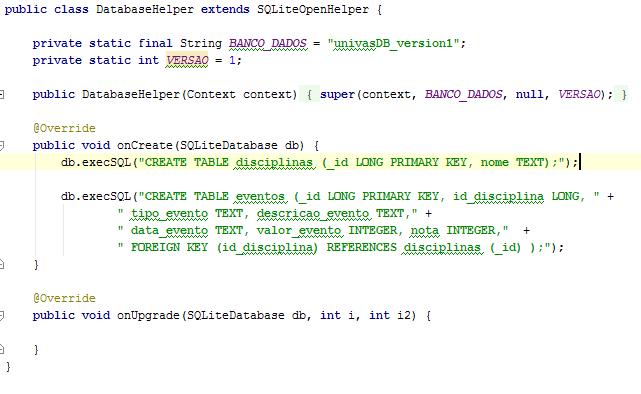
\includegraphics[scale=0.7]{./imagens/2_q_metodologico/4_procedimentos_resultados/42_aplicativo/aplicativo3.png}}
		\caption[sem legenda]{sem legenda. \textbf{Fonte:}Elaborado pelos autores.}
		\label{fig:aplicativo3}
	\end{figure}
	
	\pagebreak
	
	\par A fim de estabelecer uma conexão entre o aplicativo e \textit{web service}
foi preciso conceder a permissão de acesso à internet no
\texttt{AndroidManifest.xml} com o seguinte comando: \texttt{<uses-permission
android:name="android.permission.INTERNET" />}.

	\par Logo após, criou-se uma classe chamada de \texttt{HttpUtil} para ler
informações recebidas \textit{web service}. Nela foram inseridos dois métodos,
um para identificar as informações referentes as disciplinas cursadas e outro
para captar os dados de eventos como notas, faltas e provas agendadas. Na
Figura \ref{fig:aplicativo4} é possível ver o método incumbido de interpretar
os elementos das matérias.

	\begin{figure}[h!] 
		\centerline{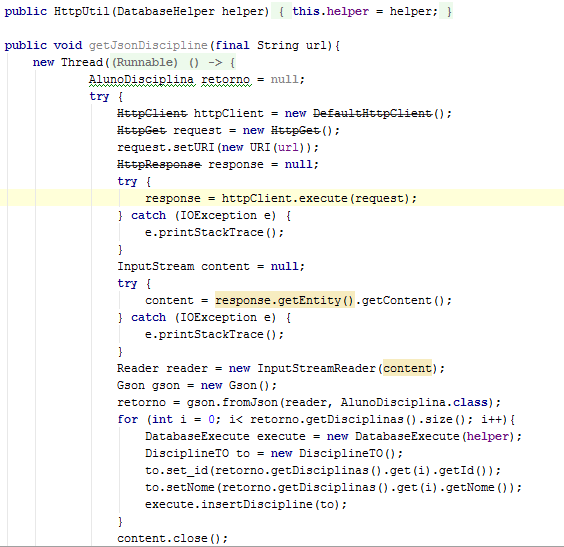
\includegraphics[scale=0.7]{./imagens/2_q_metodologico/4_procedimentos_resultados/42_aplicativo/aplicativo4.png}}
		\caption[sem legenda]{sem legenda. \textbf{Fonte:}Elaborado pelos autores.}
		\label{fig:aplicativo4}
	\end{figure}
	
	\pagebreak
	
	\par Nos métodos de leitura dos dados foi preciso criar uma \texttt{thread}
separada da \texttt{thread} principal do sistema, evitando travar a aplicação
enquanto recebe as informações vindas do \textit{web service}. Estes dados
estão em formato JSON e foi utilizado a biblioteca Gson para convertê-las no
formato esperado. Para utilizá-la foi fundamental adicioná-la como uma
dependência do projeto, conforme mostra a Figura \ref{fig:aplicativo5}.
	
	\begin{figure}[h!] 
		\centerline{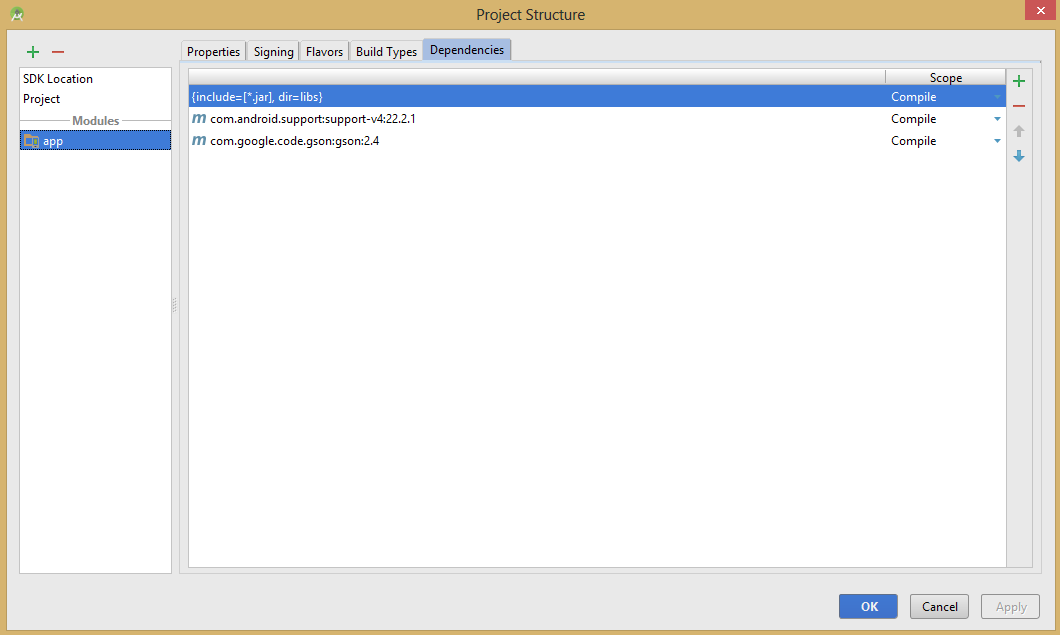
\includegraphics[scale=0.45]{./imagens/2_q_metodologico/4_procedimentos_resultados/42_aplicativo/aplicativo5.png}}
		\caption[sem legenda]{sem legenda. \textbf{Fonte:}Elaborado pelos autores.}
		\label{fig:aplicativo5}
	\end{figure}

	\pagebreak
	
	\par Ao receber as informações do servidor \textit{web} é preciso salvá-las no
banco de dados do aplicativo. Para isso desenvolveu-se uma classe chamada
\texttt{DatabaseExecute}, encarregada de inserir, alterar e buscar os dados dos
estudantes no banco de dados. Na Figura \ref{fig:aplicativo6}, pode se ver o método
pelo qual são inseridos os eventos ocorridos. Esses eventos podem ser notas, faltas ou provas
agendadas.


	\begin{figure}[h!] 
		\centerline{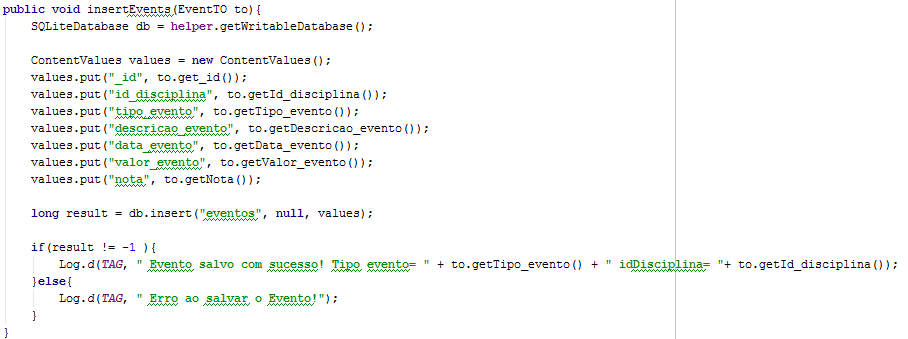
\includegraphics[scale=0.60]{./imagens/2_q_metodologico/4_procedimentos_resultados/42_aplicativo/aplicativo6.png}}
		\caption[sem legenda]{sem legenda. \textbf{Fonte:}Elaborado pelos autores.}
		\label{fig:aplicativo6}
	\end{figure}

	\par O método recebe um objeto do tipo \texttt{EventTO}. Para que seja possível
a inserção dos dados, \citeonline{monteiro2012} afirma, que é necessário
recuperar a referência da classe \texttt{SQLiteDatabase}, através do método
\texttt{getWritableDatabase()}, logo após é instanciada a classe
\texttt{ContentValues}, onde é informado o campo da tabela e o valor desejado.
Ao concluir é chamado o \texttt{insert} da classe \texttt{SQLiteDatabase}
informando o nome da tabela e o objeto da classe \texttt{ContentValues}.

	\par Para listar os resultados dos exames realizados pelos discentes no painel
de notas é utilizado o método \texttt{getResults()}, da classe
\texttt{DatabaseExecute}. Ele retorna uma lista de objetos da classe
\texttt{EventTO}. De acordo com \citeonline{monteiro2012}, para conseguir
recuperar as informações armazenadas no banco de dados é preciso adquirir a
instância de leitura da classe \texttt{SQLiteDatabase} através do método
\texttt{getReadableDatabase()}. Por meio dele pode-se realizar a consulta e
recebe um \texttt{Cursor} para navegar pelos resultados. Por fim, é composto um
objeto do tipo \texttt{EventTO} e inserido na lista. Na Figura
\ref{fig:aplicativo7} é apresentado o método \texttt{getResults()}.

	\begin{figure}[h!] 
		\centerline{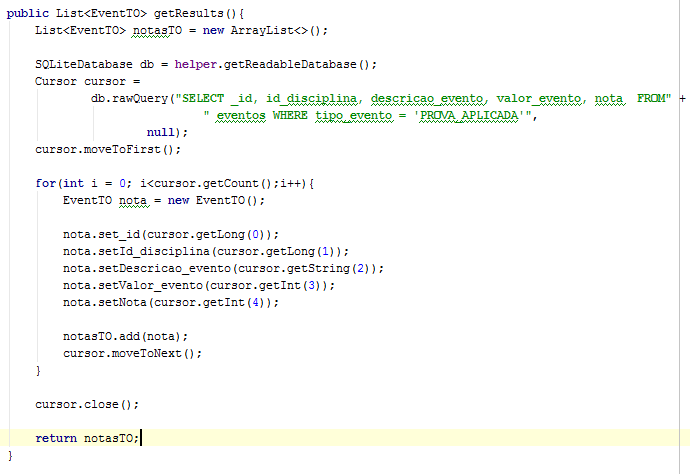
\includegraphics[scale=0.60]{./imagens/2_q_metodologico/4_procedimentos_resultados/42_aplicativo/aplicativo7.png}}
		\caption[sem legenda]{sem legenda. \textbf{Fonte:}Elaborado pelos autores.}
		\label{fig:aplicativo7}
	\end{figure}
	
	\par Para que as informações possam aparecer na tela, a classe
\texttt{ListResultsActivity} deve informar ao sistema operacional o
\textit{layout} a ser chamado através do método \texttt{setContentView()}. Por
fim, deve recuperar uma instância do \textit{widget} que apresentará os dados,
no caso \texttt{expandableListView}, e passar para a classe com função de
\texttt{Adapter} a lista de disciplinas cursadas e as notas, para que ela possa
fazer a organização das informações. Como pode-se ver na Figura
\ref{fig:aplicativo8}.

	\begin{figure}[h!] 
		\centerline{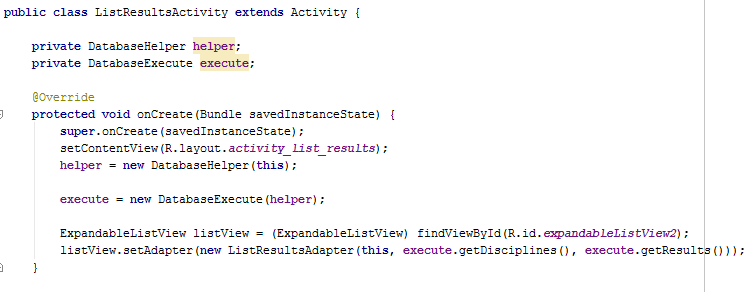
\includegraphics[scale=0.60]{./imagens/2_q_metodologico/4_procedimentos_resultados/42_aplicativo/aplicativo8.png}}
		\caption[sem legenda]{sem legenda. \textbf{Fonte:}Elaborado pelos autores.}
		\label{fig:aplicativo8}
	\end{figure}

	\pagebreak
	
	\par Na classe \texttt{ListResultsAdaper} as informações referentes as matérias
são inseridas em um vetor de \textit{string} enquanto as notas são inseridas em
uma matriz, conforme ilustra a Figura \ref{fig:aplicativo9}. Ao findar esse processo,
utiliza-se o método \texttt{getGroupView()} para apresentar os nomes das disciplinas e o
método \texttt{getChildView()} para mostrar as notas da matéria desejada, como
demostra a Figura \ref{fig:aplicativo10}.


	\begin{figure}[h!] 
		\centerline{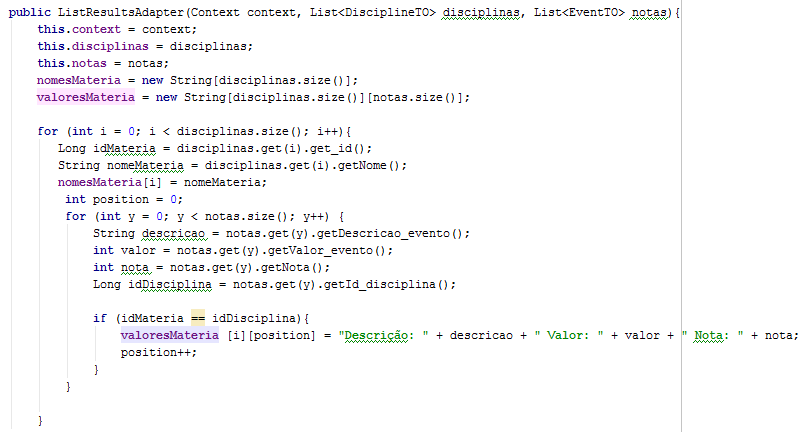
\includegraphics[scale=0.60]{./imagens/2_q_metodologico/4_procedimentos_resultados/42_aplicativo/aplicativo9.png}}
		\caption[sem legenda]{sem legenda. \textbf{Fonte:}Elaborado pelos autores.}
		\label{fig:aplicativo9}
	\end{figure}
	
	\begin{figure}[h!] 
		\centerline{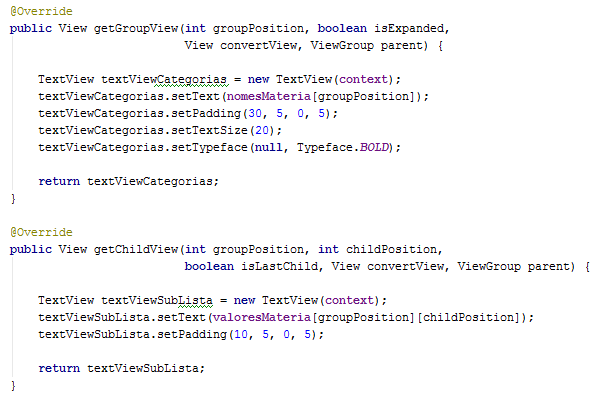
\includegraphics[scale=0.60]{./imagens/2_q_metodologico/4_procedimentos_resultados/42_aplicativo/aplicativo10.png}}
		\caption[sem legenda]{sem legenda. \textbf{Fonte:}Elaborado pelos autores.}
		\label{fig:aplicativo10}
	\end{figure}
	
	\pagebreak
	
	\par Nesse contexto, criou-se uma classe denominada
\texttt{GcmControllerUnivas}, que verifica se o aparelho em que o aplicativo
está instalado é compatível com os requisitos do GCM. Caso o dispositivo esteja
com as configurações recomendadas, é executado o método
\texttt{registerInBackground()}, para que possa gerar a chave de registro na
\textit{Google}. Ao receber essa chave é chamado o método
\texttt{sendRegistrationIdToBackend()}, encarregado de enviar esse código para
o \textit{web service}. Na Figura \ref{fig:aplicativo11}, vê-se o método
\texttt{registerInBackground()}, recebendo na variável \texttt{regid}, a chave
de registro do aparelho, realizado pela classe nativa
\texttt{GoogleCloudMessaging}, ao ser passado o id do projeto gerado na
\texttt{Google Developers Console}.

	\begin{figure}[h!] 
		\centerline{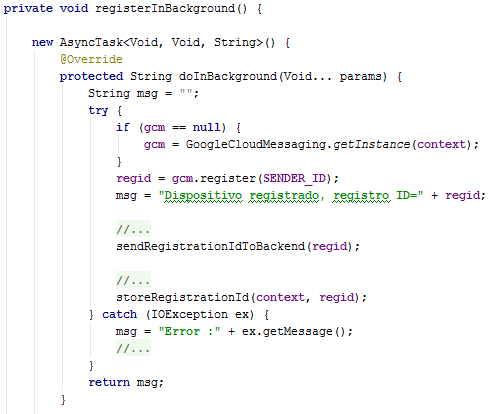
\includegraphics[scale=0.60]{./imagens/2_q_metodologico/4_procedimentos_resultados/42_aplicativo/aplicativo11.png}}
		\caption[sem legenda]{sem legenda. \textbf{Fonte:}Elaborado pelos autores.}
		\label{fig:aplicativo11}
	\end{figure}
	
	\pagebreak
	
	\par Desta forma, quando o \textit{web service} envia uma informação ao GCM, é
transmitido junto aos dados o \texttt{Registration ID}, gerado pelo método
\textit{registerInBackground()}, possibilitando ao serviço da \textit{Google},
identificar a qual dispositivo deve conduzir a mensagem.

	\par Ao receber os registros enviados pelo GCM o \texttt{broadcastReceiver}
chama a classe que apresenta ao usuário a notificação, no entanto, antes de
notificá-lo a informação recebida é enviada à classe \texttt{HttpUtil} que faz
a leitura dos dados e os salva no banco de dados. Ao findar esse processo é
analisada se a informação recebida é de notas, faltas ou provas agendadas e
chama o método \texttt{sendNotification()} que recebe um objeto de
\texttt{EventTO} e o tipo do evento.

	\par Por fim, adiciona em uma lista de \texttt{String} as informações que devem
ser apresentadas aos estudantes, passando-as para a \texttt{activity}
responsável em exibí-las. A notificação, por sua vez, é exposta através do
comando retratado na Figura \ref{fig:aplicativo12}, onde identifica-se os
atributos da notificação como a ícone que aparecerá, o título e a mensagem. O
método \texttt{notify()}, é responsável por fazer a notificação aparecer.

	\begin{figure}[h!] 
		\centerline{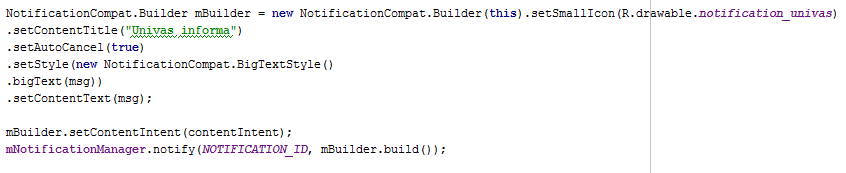
\includegraphics[scale=0.60]{./imagens/2_q_metodologico/4_procedimentos_resultados/42_aplicativo/aplicativo12.png}}
		\caption[sem legenda]{sem legenda. \textbf{Fonte:}Elaborado pelos autores.}
		\label{fig:aplicativo12}
	\end{figure}
